\documentclass[11pt,twocolumn,a4paper]{article}

\usepackage{palatino}
\usepackage[defaultmono]{droidmono}

\usepackage[english]{babel}
\usepackage[text={16cm,22.5cm},centering]{geometry}
\usepackage{marginnote}

\usepackage{listings}
\usepackage[pdftex]{graphicx}

\usepackage{enumitem}
\usepackage{caption,subcaption,float}

\usepackage{comment}
\usepackage{hyperref}

%\def\todo#1{\emph{#1}} %TODO in italics
\def\todo#1{} %TODO onzichtbaar
\def\note#1{} %TODO onzichtbaar

\def\jav#1{\texttt{\bfseries #1}}

\title{Research Plan: Towards assessment strategies for the new Dutch Computer Science secondary education curriculum.}
\author{Researcher: Renske Smetsers-Weeda}
%\affiliation{
%    \institution{Radboud University}
%    \city{Nijmegen}
%	\country{The Netherlands}}
%\email{Renske.Smetsers@science.ru.nl}
\date{}


\begin{document}

%\begin{abstract}

%Programming, where problem solving and coding come together, is cognitively
%demanding. Whereas traditional instructional strategies tend to focus on
%language constructs, the problem solving skills required for programming
%remain underexposed.
%
%
%In an explorative small-scale case study we explore a ''thinking-first''
%framework combined with stepwise heuristics, to provide students structure
%throughout the entire programming process.
%
%
%
%Using unplugged activities and high-level flowcharts, students are guided
% to brainstorm about possible solutions and plan their algorithms before
% diving into (and getting lost in) coding details. Thereafter, a stepwise
% approach is followed towards implementation. Flowcharts support novice
% programmers to keep track of where they are and give guidance to what they
%need to do next, similar to a road-map.
%
%
%
%High-level flowcharts play a key role in this approach to problem solving.
%They facilitate planning, understanding and decomposing the problem,
%communicating ideas in an early stage, step-wise implementation and
%evaluating and reflecting on the solution (and approach) as a whole.

\end{abstract}

\maketitle

\section{Introduction}\label{sec:intro}
Assessment is one of the most fundamental aspects of education, playing an integral role in teaching and learning. In particular, summative assessment can be used for gauging to which extent learning objectives are being met. Adequately determining a student's proficiency of concepts, skills and competencies is a complex undertaking. Valid, objective, reliable, and fair assessments call for a setting in which students are given ample opportunity to provide evidence of their knowledge and skills, and that a teacher can effectively observe and measure their level of mastery\todo{attainment level reached}.

Computer science is a multifaceted subject, bringing together conceptual (CS) knowledge, computational thinking, and problem-solving skills. This knowledge can be categorized as factual knowledge (knowing what), procedural knowledge (knowing how), conceptual knowledge (knowing why), and meta-cognitive knowledge (knowing about knowing)\cite{streun2001kennis}. To assess achievement levels on its crossroads is far from trivial. In addition to pedagogical and content knowledge, it requires knowledge on constructing frameworks, test specifications, and the ability to align learning objectives with assessment tasks which match specific classroom needs. This research explores the characteristic features of effective CS assessment, which incorporate the wide range of knowledge, computational thinking and problem solving skills, and what pedagogical-content-knowledge teachers need for its implementation.

\subsection{Current Situation}


As of 2019, a reformed Computing Science curriculum will become effective in the Netherlands. The reformed program follows in the footsteps of recent international reforms (examples are the U.S. CSTA, U.K. National curriculum, New Zealand's new "Digital Technologies") where a shift from computer and ICT applications towards rigorous computing has taken place. \citeA{Brown2013} report on challenges and successes of implementation in the UK. \citeA{Bell2014} discuss issues that teachers face after New Zealand's new standards were introduced in 2011. On another continent, \citeA{Yadav2016} discuss the implications and challenges on CS teachers in the Unites States.

In the Netherlands, the reform has resulted in a stronger focus on fundamental concepts, including analysis of standard algorithms and being able to compare efficiency and implementability \cite{Barendsen2016}. Higher-order (Computational Thinking) skills are positioned as a fundamental pillar, characterized as one of the 21st-century skills competencies (\cite{SLO2015}). The idea of Computational Thinking (CT) presents a different way of thinking about computing proficiency by emphasizing the (problem-solving) skills that students need to solve complex real-world problems and evaluate proposed solutions. It also implies that solely measuring CS proficiency as the acquisition of core content knowledge no longer suffices \cite{Yadav2015}. Despite the proliferation of CT-focused programs throughout several curricula around the world, there is still no general method\todo{Erik: is die er wel in andere vakken?} on how to develop CT assessments reliably and easily \cite{catete2017framework}. In their extensive review study, \citeA{LyeKoh2014} find a few studies that have examined computational skills as outcomes. No studies were found focussing on upper secondary high school. We were able to locate one: \citeA{Lee2011}. All-in-all, little research has been done on the effectiveness of the assessment materials available \cite{Yadav2016}.
%How will this fundamental shift evolve (in) the Dutch educational landscape?\todo{Erik: kopje? wat bedoel je hiermee Erik?}




Currently, only a small percentage of the Dutch CS teachers has completed a full academic qualification to teach the subject \cite{tolboom2014informatica}.

New curricular material comes with new misconceptions. \citeauthor{duncan2017teachers}'s results confirm their concern and warn that insufficiently prepared teachers may not pick up student misconceptions, or may even introduce incorrect ideas themselves. Speculating on their content knowledge (as a component of the PCK), Dutch teachers currently focus primarily on designing and implementing computer systems and programs \cite{Schmidt2007}, rather the more fundamental underlying concepts which the new curriculum now focusses on. In the Netherlands there is no centralized or standardized exam for the subject, no validated assessment tasks, and no way to ascertain the effectiveness of teaching. Teachers must develop their own assessments. From their community of practice observations, \citeA{hermansen2014reworking} conclude that teachers create their own assessments, generally by adapting others. There is usually only one teacher in a school, leaving them isolated from their peers. Compared to initiatives such as the U.K. Computing At School (CAS), professional development opportunities, communities of practice, sharing of experiences, resources, and lessons learned are sparse. All in all, teachers have no assessment benchmark, and lack valid and reliable example assessments \cite{Yadav2015}, and furthermore lack evaluation or reflection on their teaching strategies via peer-collaboration. In their research, \citeA{GroverPea2013} describe that paying attention to assessment is a pre-requisite to successful implementation of any curriculum and conclude that large gaps exist pertaining to assessment. Denning \cite{denning2017remaining} notes that educators internationally have many basic questions about teaching and assessing CT and expresses his concerns for ineffective teaching. Along the same line, \citeA{2013Seiter} describes assessment models incorporating progression pathways as vital for establishing research-based computational curricula.


There is a gap between the (meager) research and classroom practice\cite{Yadav2015}. Computing education and research suffer from the lack of assessment instruments\cite{voogt2017effecten}. In their research \citeA{2010TewGuzdial}, argument the importance of validated assessment that could be widely applicable across tertiary curricular approaches. This need may be even more true for secondary education, where far less relevant research has been done in the first place. Also, research developments are not accessible to teachers (either they need a paid subscription, academic literature may be written incomprehensibly, or not practical as it can't be implemented in the classroom in a cost-effective manner). What is needed are validated assessments which are of high quality, sound, scientifically grounded, yet which can be implemented in a practical manner in a classroom setting.

With all these factors in place, what is needed for teachers and their PCK to adapt to, and successfully implement, the curriculum reform?


\section{Background}\label{sec:background}
%
%\subsection{Curriculum Reform}
%As previously mentioned, CS curricula are being reformed globally.
%
%





\subsection{Computational Thinking}

There is no general consensus on the definition of Computational Thinking (Yadav, 2015). Voogt et al (2015) call for a flexible and pragmatic approach and use operationalization of CT, such as has been done by Yadav (2015). Computational Thinking refers to thought processes that are involved when solving complex problems and generalizing and transferring this problem solving process to a wide variety of problems (Voogt et al 2015). CT are higher-order-thinking skills  (Yadav2017 CT for educators) and considered an extension of every child's analytical ability (Wing 2006)(Voogt et al 2015).


Wing (2006) identifies the following CT skills:\label{CTdefWing}
\begin{itemize}
\item Algorithmic Thinking: thinking in terms of rules, steps and repetitions (of subtasks
\item Decomposition: Breaking a problem into sub-problems (which can be dealt with individually)
\item Abstraction: simplifying a problem by leaving out (unnecessary) details
\item Generalization: finding patterns and re-using solutions (transfer)
\item Evaluation: Does my solution solve the problem? Analysis: How could process/solution have been improved?
\end{itemize}





Several studies report an evident link between programming and CT (Davies, 2008)(Hu, 2011)(Crick, 2017)(Yadav et al., 2017).


%In a survey of program understanding, von Mayrhauser and Vans
%(1994) summarise studies (in particular Guindon, 1990) noting that experts:
%have efficiently organised and specialised knowledge schemas; organise their
%knowledge according to functional characteristics such as the nature of the
%underlying algorithm (rather than superficial details such as language syntax);
%use both general problem solving strategies (such as divide-and-conquer) and
%specialised strategies; use specialised schemas and a top-down, breadth-first
%approach to efficiently decompose and understand programs; and are flexible in their approach to program comprehension and their willingness to abandon
%questionable hypotheses.[Robins, Rountree, Rountre (2003).  ]


\subsection{Algorithms, Algorithmic Thinking, and Problem Solving}

Algorithms is a fundamental CS concept. Algorithms are tools for developing and expressing solutions to computational problems (Grover and Pea, 2013). To be successful in developing novel algorithms that solve problems correctly and successfully, calls for a coherent set of skills and knowledge.
On the one hand, algorithmic thinking (as part of CT) and problem-solving skills are essential (Lister et al, 2004). On the other, fundamental knowledge of the concepts of algorithms are needed, i.e., how algorithms work, which common algorithms and plans exist, and knowledge about strategies for composing (or combining) algorithmic components. CT thought processes are involved in formulating problems so their solutions can be represented as computational steps and algorithms (Aho, 2012). 

\note{CT learning takes place during programming (Brennan and Resnick, 2012)(Lye and Koh, 2014).}


\todo{How to develop skills and reinforce knowledge related to algorithms… either through concepts or programming. <SEE VERHAAL VAN DENNING, 2017>}


McCracken et al. (2001) describe five iterative steps to problem solving (abstracting, generating sub-problems, implementing sub-solutions, integrating sub-solutions, evaluating and iterating) and encompass the CT skills as defined by Wing (algorithmic thinking, abstraction, decomposition, generalization, evaluation) described by Wing (2006). The step of integrating sub-solutions (via abutment, merging and nesting) corresponds with algorithmic thinking, as it includes involves creating an algorithm that controls the sequence of events. An important aspect of it's opposite step, generating sub-problems, is recognizing plans, existing methods or strategies. Recognizing plans at an abstract level helps decompose the problem and simplifying the problem. What is left behind is to fine-tune the plan to the specific situation and then integrate it with the remaining sub-solutions.


\subsection{Assessment best practices}

A substantial amount of research has been done to role of assessment in education. In his study Frederiksen (1984) describe assessment as a motivator for learning. Alderson and Wall (1993) and Prodromou (1996) elaborate by stating that what is assessed strongly influences what is learned. Biggs (1996) prescribes that instruction, learning and assessment must be well-aligned. This alignment exists in most traditional knowledge-based tests, yet constructive alignment for competency-based instruction is not self-evident (2006Baartman). With the emphasis of Computational Thinking and problem solving in reformed CS curricula, learning and instruction is increasingly competency-based. Assessment of competencies is complex, mainly because it comprises a multi-facetted blend of knowledge, skills and attitudes (Van Merriënboer, Van der Klink and Hendriks, 2002).

\subsubsection*{Assessment Criteria}\label{sec:qualityCriteria}
Baartman et. al. (2006) proposes a 'wheel of competency assessment' framework of quality criteria for competency assessments which integrates different assessment methods into a Competency Assessment Programme (CAP). It constitutes both fit-for-purpose quality criteria (i.e. alignment, transparency, authenticity, \ldots) as well as fit-for-use utility criteria (i.e. cost and efficiency). The framework has been extended by Catete (2017) with classical psychometric quality criteria of validity and reliability. This adapted framework has recently successfully been applied to establish quality-assured programming rubrics for AP CS Principles (2017Catete).
\note{2017Catete geeft een mooi overzicht van de aspecten van de wheel, pg 100} Yadav (2015) expresses availability and ease of access an additional feature.




\subsubsection*{Design methods}

In his work, Hermansen (2014) suggests that teachers should work collaboratively on transforming (rather than implementing) assessment tasks. Such a development and refining process yields assessments specific to local settings, adhering to the needs, knowledge, skills and interests of their own students.

The Dutch curriculum description includes high-level goals (Barendsen et al. 2016). However, this description is not specific enough for the assessment. Concrete learning outcomes including the level of comprehension (taxonomy) need to be established. A similar situation exists in the UK national curriculum. The levels from the previous ICT curriculum have been removed, leaving assessment at KS3 to the responsibility of individual schools. CAS members (in co-operation with CAS Master teachers, teachers and academics) have taken the initiative to establish computing progression pathways and rubrics to assess learners' Problem-solving and Computational Thinking capabilities. With it, learning objectives and potential evidence observations have been established, yet seems to miss concrete alignment with potential works products. Importantly, Giordano (2015) concludes that designing questions clearly linked to the competencies is perceived as the most difficult task in the assessment process. Moreover, the more authentic and realistic, the more complex the detailed mapping to the abilities/competenties becomes. These is very relevant as the curriculum specifies a concept-context approach to learning. This authentic learning approach encourages students to connect real world problems to the subject matter at hand. In their paper, Goode (2014) emphasize why this makes sense: "engaging students in the context of complex, meaningful projects that require sustained engagement, critical thinking, collaboration, management, communication, and management of resources to develop final products or presentations builds the types of 21st century skills advocated by new sets of national standards". Especially when dealing with more complex tasks, explicit alignment between learning objectives, observations and work products must be established.

%\subsubsection*{Learning objectives and FKSAs}
\todo{ Naar achtergrond met meer toelichting, uitleggen. What is abilities (niet attitutes?)? What is verschil tussen skill en abilities?}
\todo{Why needed}


\note{knowledge, skills or other attributes}
%
%linked to evidence-eliciting-performances



\textbf{Evidence-Centered Design}\newline
Initiatives in the U.S. follow a different, rather structured, path, incorporating validity evidence into an assessment design process. SRI launched a Teacher Assessment Literacy for Exploring Computer Science study to investigate the design and delivery of high-quality assessment literacy materials. They use an Evidence-Centered Design (ECD) method. ECD is a principled method for modeling domains for assessment purposes that is especially useful for hard-to-assess practices (Grover, 2016). Its systematic structure facilitates a coherent mapping from high-level curricular goals to observable behaviors. This yields three models which elicit evidence of students' achievement levels of learning objectives. The student model specifies the knowledge, skills or other attributes (KSA) to be assessed. The evidence model describes observable behaviors or performances which may provide evidence about the knowledge or skills to be measured, and thus links the chain of reasoning from
students’ performances to their knowledge and skill. The task model describes ways to elicit data that provide evidence about student. Evidence is obtained by deliberately putting students in those situations, challenges, or tasks that will elicit the desired FKSAs (Grover and Bienkowski, forthcoming).






\note{Evidence models
lay out the argument about why and how observations in a given task
situation constitute evidence about student model variables. There are
two parts to an evidence model, the evaluation component and the
measurement component.}

This methodology has been used by, extensively reported on, and cited to by Mislevy et. al. (2002, 2003). It has recently also been in CS used by Grover (2017), Snow (2017), and for the development of assessment instruments for the Exploring Computer Science curriculum, as described by Mislevy (2006) and McGee (2018)\todo{[2018McGee CS outcomes]}.



\begin{figure*}\label{fig:ECD}
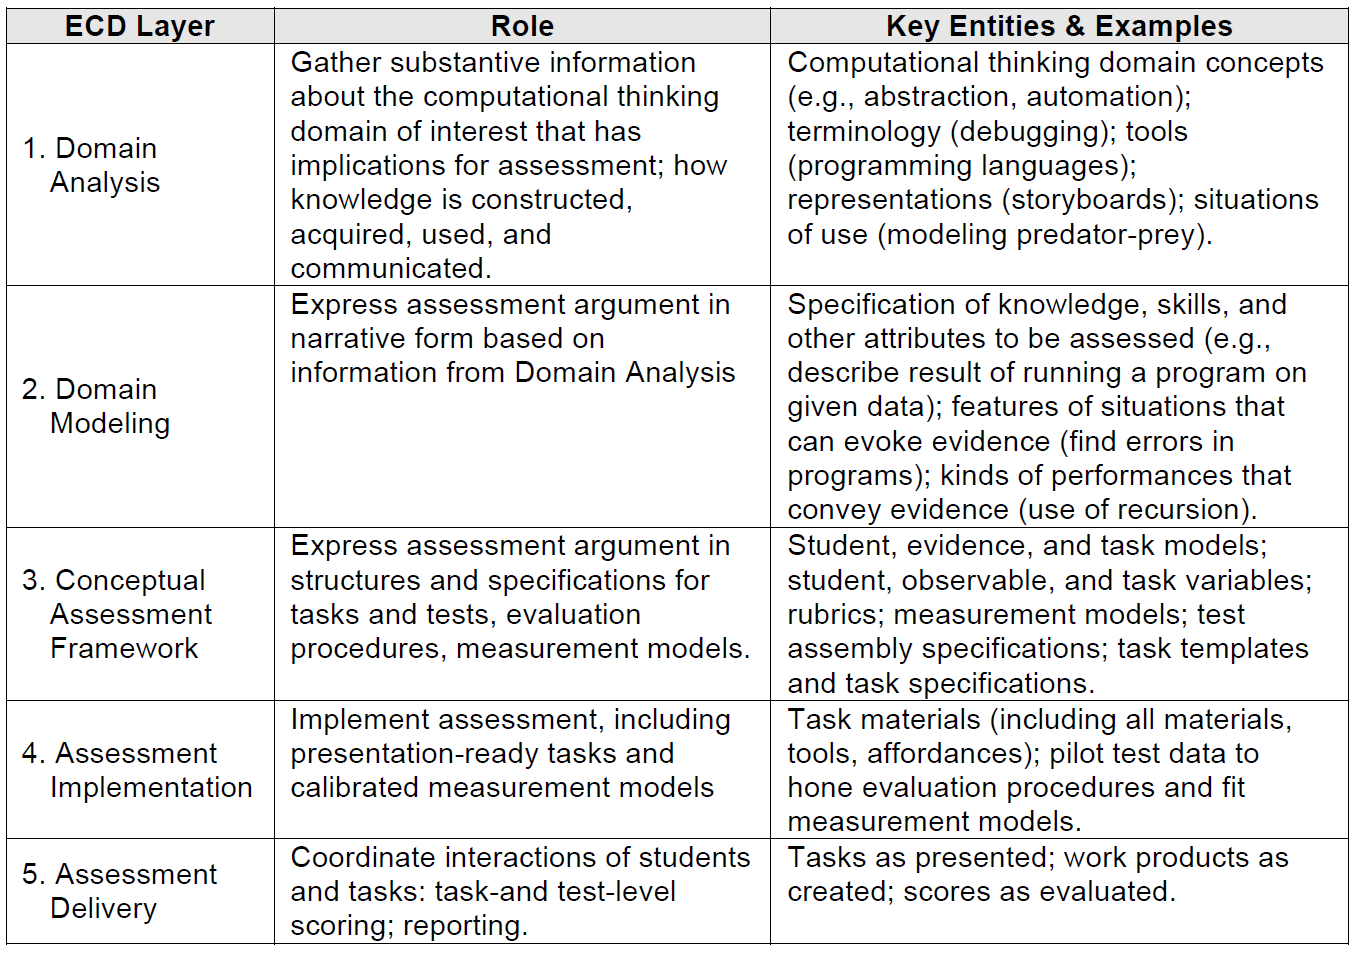
\includegraphics[scale=0.6]{figures/ECDoverview.png}
\caption{Roles and Key Entities in the Five Layers of Evidence-Centered Design (2014SnowBienkowski)}
\end{figure*}



%\begin{itemize}
%\item \textbf{Domain Analysis:}
%The top layer in the ECD process is a Domain Analysis to clarify learning goals.
%This level includes determining relevant concepts and terminology,(e.g. abstraction, algorithms), tools (i.e. programming languages) and representations (flowcharts, pseudocode) as well as understanding how knowledge is constructed, acquired, used and communicated (SRI Assessment Design Patterns for CT, 2017). In the process, the curricular learning objectives are translated into more specific and learning goals specified in operational terms, ready for teacher use
%\item \textbf{Domain Modelling:} the assessment argument was designed. The learning goals were translated into the specific focal knowledge, skills, and attributes (FKSAs)
%
%\item \textbf{Conceptual Assessment Framework:}
%The result of this phase was a design pattern consisting of three aligned models (student model, evidence model, and task model) which together form the assessment specifications: the foundation for the new assessment.
%
%\item \textbf{Assessment Implementation:}During the implementation stage, the model assessment tasks are translated into classroom-specific assessment tasks in the designated programming language.
%
%\item \textbf{Assessment Delivery:} the tasks are administered to students.
%\end{itemize}


Transitioning from one ECD layer to the next involves analytical precision and careful reasoning. To validate this step, Catete (2017) uses an expert panel. Several methods can be used to resolve any differences in opinions and obtain an object consensus between panel members, such as focus groups\todo{ref WIPSCE artikel over thresholds}, Nominal Group Technique\todo{Adler, M. & Ziglio, E. Gazing into the oracle: The Delphi method and its application to social policy and public health. Jessica Kingsley Publishers, 1996.} or the Delphi method\todo{ref brooks 779}.




\todo{Methode geven om meningsverschillen plat te strijken.  DELPHI?? De moeite waard? Misschien delen van DELPHI methode gebruiken? Kijk evt naar artikel over thresholds WIPSCE, evt met een focusgroep (is sneller en minder zwaar aangezet). Beschrijf hier hoe je verschillen gaat oplossen. Relateer evt ook aan ECS ECD met DELPHI. Elementen van methode gebruiken, niet hele methode, Nominal Group Technique? (zie 2017 catete.}





\subsubsection*{Taxonomies}

Taxonomies can be used to provide a language for describing learning outcomes and
performance in assessments, dividing them into domains (such as cognitive, affective, and psychomotor) or categories based on complexity of the task. Two widely used taxonomies for assessment of learning are the (revised) Bloom
taxonomy and the SOLO taxonomy. Both have been used in CS education research (revised Bloom: Whalley et al., 2006 and SOLO: Lister et.al 2006).


However, it has been reported that there are some drawbacks to their use in CS. Thompson et. al. (2008) report that experts have difficulties applying Bloom's taxonomy consistently in introductory programming courses. The classification becomes meaningless as all tasks seem to fall into the same category. Given the difficulties in categorizing programming activities within the existing taxonomies, several attempts have been made to propose new taxonomies appropriate for CS education.

\note{In part this is because the terms synthesis and evaluation are not useful in describing programming learning outcomes.} Fuller et. al. (2007) explain that though SOLO can be used for holistic marking, it says nothing about the type cognitive processing, such as recalling items or drawing conclusions. They suggest to separate Bloom’s levels into two dimensions, producing (writing) and interpreting. Lister and Leaney (2003) attempt to differentiate in terms of magnitude of the code.

Meerbaum-Salant et. al. (2013) propose a hierarchical taxonomy scale describing how student’s performance grows in complexity. It’s aim is to pinpoint (the development of) programming skills: both problem solving (such as plan composition) and (construct-based) language aspects. It is based on a combination of the Revised Bloom and Solo taxonomies. The result is a nine-level taxonomy with
the highest level being relational creating, and the lowest level being
unistructural understanding (on one axis: understanding, applying, creating; on the other: unistructural, multistructural, relational)\todo{ Erik: Laat de lezer de taxonomieen zien, evt met figuren (wat meer toelichten)
}:


%Meerbaum-Salant et. al. (2013) propose a hierarchical taxonomy
%scale based on a combination of the revised Bloom and Solo taxonomies
%\cite{Meerbaum2013}. Three super-categories - unistructural, multistructural,
%and relational (derived from the Solo taxonomy) were chosen, each containing
%three sub-categories - understanding, applying, and creating (derived from
%the revised Bloom's taxonomy:

\begin{description}[leftmargin=1em]
\item[Understanding:] The ability to summarize, explain, exemplify,
    classify, and compare CS concepts, including programming constructs.
\item[Applying:] The ability to execute programs or algorithms, to track
    them, and to recognize their goals.
\item[Creating:] The ability to plan and produce programs or algorithms
    (constructing, analysing, evaluating and formulating).
\item[Unistructural:] The ability to create very small scripts doing one
    thing, or adding an instruction with a local effect to an existing
    script.
\item[Multistructural:] The ability to track a program and grasp various
    parts but not the entity they form as a whole.
\item[Relational:] The ability to fully understand a complex concept (such
    as concurrency) and to coherently explain its various facets.
\end{description}






\subsubsection*{Identifying levels of mastery}
A substantial body of work has previously explored the assessments used in novice programming courses in tertiary education (Luxton-Reilly, 2018)\todo{mer woorden gebruiken, uitleg vanuit docenten stoel}. In prior work, researchers claimed that the subject itself was difficult. McCracken et al. (2001) discuss how students fail to complete tasks, and Robins, Rountree, Rountre (2003) associate it with high dropout rates in introductory programming courses.  However, more recently, assessment tasks were found to be more complex than academics expected (Whalley, Lister et al., 2006; Luxton-Reilly, 2018)\todo{geen twee refs achter elkaar}. For example, tasks typically require both algorithmic thinking (initialize before changing), as well as a more advanced understanding of data representation (assigning a value to a property)(Seiter, 2013).

Assessment tasks should adequately indicate a students’ programming comprehension and clearly discriminate between achieved performance levels. Predicting the difficulty of programming tasks and understanding alternative conceptions has shown to be difficult (Lonati, 2017)\todo{ Toelichten: bv een invulopgave kan op verschillende manieren aangepakt worden}. In their findings, Oliver et al., (2004) indicate that introductory and intermediate programming courses assess at a constant level of difficulty and restricted solely to Bloom’s application and analysis level. The inability to accurately measure student performance may well contribute more to the poor results highlighted in several studies (such as the McCracken et al, 2001) than failures of student comprehension [2010TewGuzdial].  In their paper, Whalley et al. (2006) also relate the high failure rate in introductory programming courses to unfair and inappropriate assessment instruments, especially for non-elite institutions.




However, whatever taxonomy chosen, scientists agree that classifying tasks is far from straightforward (Fuller et al., 2007; Thompson, Luxton-Reilly, Whalley, Hu, and Robbins, 2008). As a result, researchers exclaim that "the pattern of achievement is not clear" (2013Zur-Bargury), making their analysis difficult and inconclusive. Maybe the issue is not the taxonomy, but rather the task being classified.

In their research Luxton-Reilly (2018) state that “most assessments used in formal examinations combine numerous heterogeneous concepts, resulting in complex and difficult tasks”. We agree that difficulty that experts endure whilst trying to classify the tasks (Meerbaum-Salant et al, 2013) is related specifically to the nature of the tasks. De Raadt et al. (2009) explains that the identification, selection and application of plans which can be seen as a representation for strategy (similarly described by Soloway (1985), also known as patterns (Wallingford, 1996)). They distinguish a set of elementary plans (programming strategies) that can be combined to create a solution. Soloway (p. 856) and de Raadt identify the following methods of integrating plans (bottom-up):
-	Abutment: plans following each other in sequence. For example, initializing a variable and printing it’s value (i.e. x=12; print(“The value of x is: “, + str(x) ) )
-	Nesting: one plan as a whole is submerged in another. For example, printing the value of a variable is constituent to a counting plan.(i.e. counter=0; while not done counter ++;print(“The number of items is: ” + str(counter)) )
-	Merging: interleaving (at least) two plans. For example, in the averaging problem, the input, summing and counting plans are merged.


Examples are Initialization plan (variables), Average plan, Triangular Swap plan, Guarded Division plan, Counter-Controlled Loop plan, Sum and Count plans, Bubble Sort algorithm.

Strategies can be expressed both simply, at a sub-algorithmic level, and at a higher level which are found in solutions produced by expert programs (de Raadt, Toleman and Watson, 2006). A number of attempts have been made to decompose these strategies (Muller, Haberman, and Ginat, 2007; Porter and Calder, 2003; Wallingford, 2007) \todo{ Erik: uitsplitsen en toelichten wat ieder gedaan heeft zodat je dit als lezer niet zelf hoeft op te zoeken }into  smaller units and distinguish pre-requisite knowledge. These plans and higher level algorithms map to multi-structural and relational levels in the SOLO taxonomy. In their combined efforts, Luxton-Reilly et al. (2018) have managed a first step towards decomposition, by for example recognizing and identifying initialization, use of conditionals and nesting.  \todo{ Erik: Zhong hier relevant over task?}




Cross-referencing, we see that Luxton-Reilly et al.’s top-down approach in which they decompose a complex task does not systematically consider all concept combinations and thus sources of difficulties and alternative conceptions. For example, in their nesting-task, they fail to recognize \todo{nuanceren}that a student may not understand the difference between a loop nested in a conditional and a conditional nested in a loop. De Raadt et al. is also not complete, missing the idea of procedures, functions, parameters, and a Boolean-Flag loop plan as a specific form of a primed sentinel controlled loop plan. Here too we see that underlying concepts at a unistructural level are left out\todo{nuanceren}. For  example the very first plan, the average plan, explicitly states the need to understand the division operator, but not the assignment of variables .

In his work, Lister (2010, 2016) positions the Piagetian and neo-Piagetian theories. The Piagetian theory describes how students may reside in different stages of cognitive development for each fundamental concept being taught. The neo-Piagetian theory extends this with the idea with an ”overlapping waves” model, a novice programmer can reside in multiple stages simultaneously. The stages coincide with those of the SOLO taxonomy. In their paper, Szabo et al. (2014) propose a curriculum analysis methodology based on Neo-Piagetian theory to facilitate lecturers in tracing the development and assessment of concepts throughout their courses. This theory describes how students may reside in a different stages of cognitive development for each fundamental concept being taught. CAS has developed Computing Progression Pathways (Dorling and Walker, 2014) to identify the major knowledge areas (concepts) and CT skills of computing and provides specific indicators of increasing levels of mastery (e.g. distinguishing between ‘understands’ and ‘can apply’) of the subject in those areas (Giordano, 2015  ).\todo{ Erik: Licht toe en zet tegen elkaar af: “de ene onderzoek maakt wel onderscheid tussen verschillende… maar niet…”} \todo{ Nesten is een complexiteit op zichzelf
“Afhankelijkheid is geen onderdeel van de onderzoek van… “}

Summarizing, the introduction of the new computing curriculum could benefit from tooling which aids the establishment of assessments. Teachers will and should create assessments tailored specifically to their classroom needs, but lack specific PCK to do so. Not only is creating a qualitative assessment acknowledged as a difficult task, in this particular case, teachers must first acquire and internalize knowledge about the new concepts and may not yet have reached the desired final level.





\subsection{Assessment Techniques}
Assessments are used for several purposes. McMillan (2007) distinguishes between two types of assessments, summative and formative. Summative assessment refers to the use of assessment-based evidence to help us arrive at go/no-go decisions based on the success of a completed course or instructional program (Popham, 2009). On the other hand, assessment for learning is formative. Formative assessment is used by both students and teachers to adjust ongoing instructional and learning activities in order to improve the manner in which learning is taking place. Summative assessment can also be treated formatively, for example to determine the effectiveness of instruction.


\subsubsection*{PCK}

Effective teaching requires a combination of pedagogy, content, and knowledge (PCK) (Shulman, 1986). In a nutshell, it means that subject matter (content knowledge) and ways of teaching (pedagogical knowledge)(Yadav, 2016) are integrated. It encompasses about knowing what makes certain topics easy or difficult, as well as ways of representing and formulating topics in different ways (Shulman, 1986).

Magnusson, Krajcik en Borko (1999) distinguish four aspects of content-specific PCK: knowledge of
(1) curricula, (2) students' understanding and difficulties, (3) instructional strategies, and (4) assessment.


In this research we focus on one aspect of PCK, namely assessment. \todo{and are particularly interested in the PCK aspects needed to adapt and implement particular types of assessment}


\subsubsection*{Assessment as a part of PCK}
Very little is known about PCK for Computing (Yadav, 2016). As a part of PCK, teachers have limited knowledge about assessment and seriously struggle with it (Popham, 2009). Particularly, teachers face many challenges with respect to the assessment of new topics (DeLuca and Klinger, 2010). The 2015 study by Computer Science Teacher's Association (CSTA) found that teachers face a number of challenges finding valid and reliable assessments to use in their classrooms. Along the same line, Dutch teachers say they lack qualitative (peer-)reviewed materials, assessment rubrics and question banks (Tolboom et al., 2014). Yadav et al. (2015) conclude that teachers lack PCK, which manifests itself in an incapacity to act: teachers understand need for qualitative assessment, but just don't know how to.

%Both experienced and novice teachers struggle in assessing student learning (Fincher, Kolling, Utting, %Brown, Stevens 2010)(Hebert \& Worthy, 2001)(Veenman, 1984) (Yadav, 2016)(Yadav, %2015)(Bardensen et al., 2015 ITICSE wg).

Faced with a specific assessment task, teachers generally take previously developed templates as a point of departure and adapt them to meet their current requirements (Hermansen, 2014). During his observations he saw that teachers spent significant time on aspects related to eliciting evidence of students' approach to a task. This indicates that teachers are well-informed about the role of an assessment.
Particularly, teachers face many challenges with respect to the assessment of new topics (DeLuca \&Klinger, 2010). The 2015 study by Computer Science Teacher's Association (CSTA) found that teachers face a number of challenges finding valid and reliable assessments to use in their classrooms. Along the same line, Dutch teachers say they lack qualitative (peer-)reviewed materials, assessment rubrics and question banks (Tolboom et al., 2014). Yadav et al. (2015) conclude that teachers lack PCK, which manifests itself in an incapacity to act: teachers understand need for qualitative assessment, but just don't know how to. To elicit: CS teachers assess merely a small spectrum of levels in Bloom's taxonomy, ascertained by Oliver et al. (2004) and confirmed by Whalley et al. (2006). Depending on the particular concept, in some cases only the lower knowledge levels are assessed (networks), in others predominantly the higher application and analysis levels (programming). Either way, this leads to non-discriminative assessments. Even if there is published material available, many teachers create and rely on their own material (Popham, 2009).

Thus, judgements about students' proficiency are made without the use of validated assessments. If the quality of assessment is insufficient, the teaching will be ineffective (Ragonis, 2012).  If teachers use low-quality assessment instruments we will end-up teaching the wrong subject; and vice-versa (Giordano et al., 2015).  Whalley et al., (2006) describe the assessment of programming as complex and challenging and emphasize the lack of clear frameworks and tools.





In his review on developing generic resources for assessment, Hermansen (2014) concludes, based on several researches (Coburn, 2001, 2003; Edwards, 2008; Horn \& Little, 2010; Hutchinson \& Hayward, 2005; Rasmussen \& Ludvigsen, 2009; Tierney, 2006), that assessment tools aren't plug-and-play modules that remain instantaneously operable after a relocation. Rather, they must be adapted  and 'recontextualized' according to classroom needs. From his review he summarizes that teachers who implement formative assessment resources "draw upon a strong understanding of subject knowledge, use a range of ideas and tools to enable classroom interaction and learning, have established a new division of labour in their classrooms, focus on developing student learning and autonomy, and critically examine their own beliefs about learning and classroom practices" (Black \& Wiliam, 2006; Brookhart, Moss, \& Long, 2010; Harrison, 2005; James \& Pedder, 2006; MacPhail \& Halbert, 2010; Suurtamm et al., 2010; Webb \& Jones, 2009; Willis, 2011). This list alone affirms that any teacher new to a particular concept, or new at all to teaching, will likely be lacking some, if not all of these skills or knowledge.


Teacher educators need to provide teachers with the content, pedagogy, and instructional strategies needed to incorporate computational thinking, and in particular the assessment of the its core concepts (Yadav2017).



\subsubsection*{CT assessment}
With the lack of a precise definition as one of its contributing factors, Computational Thinking is perceived to be one of the more challenging concepts to teach and assess (2017Crick).

There is no clear definition of CT(Crick, 2017) making it difficult to assess. Recently some research into assessment of Computational Thinking has been published (Yadav, 2017)(Yadav, 2016). Evaluating CT is perceived as difficult (Brennan and Resnick, 2012) (Crick, 2017).
Without rigorous assessment, computational thinking cannot be successfully embedded in education (Grover et al., 2014).

Grover et. al. (2017) call for measures that enable educators to assess student learning of CT.  Specifically they signal the necessity to test and validate materials in various settings with diverse learners.
Assessments of CT remain underdeveloped and under-researched (Yadav et al., 2015).
Educators need a manner to assess and validate what CT a student has learned (Grover and Pea, 2013).
In their review study, [2014LyeKoh], summarize that of the research on computational thinking through programming , stunningly none focus on upper secondary high school (ages 15-18) (but merely on elementary or higher education).


\subsubsection*{Algorithms assessment}
Poor CS1 results: Lister, McCracken


The 2001 ITiCSE report by the McCracken Group (McCracken, 2001), a keystone in assessment literature (Giordano, 2015) on CS concepts, describes the difficulties pertaining to the development and validation of assessment activities. They raise concerns about task selection and the difficulties of standardizing assessments for multiple institutes.

\subsubsection*{Fit-for-purpose assessment tasks}
CS1 much research to assessment tasks: mc, parsons, sniplets,


meet the criteria in \ref{sec:qualityCriteria} in addition

\subsection{Black hole: Assessment in Secondary CS education}
There is a gap between the (lean) research and classroom practice (Yadav, 2015). All-in-all, little research has been done on the effectiveness of the assessment materials available (Yadav,2016). Computing education and research suffer from the lack of assessment instruments (Voogt et al., 2017). In their research [2010TewGuzdial], argument the importance of validated assessment that could be widely applicable across tertiary curricular approaches. This may be even more true for secondary education, where far less relevant research has been done in the first place. In addition, research developments are not accessible to teachers (either they need a paid subscription, academic literature may be written in an incomprehensible manner, or not practical as it can’t be implemented in the classroom in a cost-effective manner). Recent published work based on CT have a focus in primary education or middle school(review studie LyeKoh 2014). Research based on (the assessment of) CS concepts has a focus on tertiary education (such as McCracken 2001, TewGuzdial 2010). Merely a few studies focus on CS concepts or CT specifically in secondary education.





\section{Aim of the thesis}\label{sec:aim}
All-in-all, little research has been done on the effectiveness of the assessment materials available \cite{Yadav2016}. Recent published work based on CT focusses on primary education or middle school \cite{LyeKoh2014}. Research based on (the assessment of) CS concepts has a focus on tertiary education (such as \cite{McCracken2001},\cite{2010TewGuzdial}). More specifically, we know little about how teachers are to assess specific CS concepts or computational practices pertaining to Algorithms and Physical Computing in secondary education.

The aim of this thesis is to contribute to the knowledge about assessment pertaining to the domains of algorithms, physical computing and their related computational practices and typifying which PCK it demands from teachers to assess these domains.
%and what PCK is requires/demands/involves from teachers
%knowledge domains of algorithms, physical computing and the related computational practices.
%en vertalen we naar...

\subsection*{Algorithmic task difficulty}
Section \ref{sec:researchAssProgramming} describes that despite efforts from the research community, creating programming assessment tasks that measure what we wish to measure, especially with respect to difficulty, remains a challenge. It was outlined that several researches attempt to classify tasks according to task-oriented features, however do so without isolating the elementary concepts from the strategies, and as a result try to assess (nested) concepts and (problem-solving) strategies simultaneously. Determining task difficulty could be facilitated by clearly separating conceptual knowledge from computational practices (as proposed by \citeauthor{BrennanResnick2012}). As proposed by \citeauthor{deRaadt2009teachingPlans}, plans could be integrated into tasks order to assess strategies. To our knowledge, there has not yet been an attempt to systematically untangle assessment tasks by focussing on computational practices and in doing so, isolating and identifying not only elementary programming concepts but also algorithmic components \cite{deRaadt2008}. The focus lies specifically on the fundamental CS concept of algorithms and the closely coupled algorithmic thinking (as a part of CT) and problem solving skills. The choice for a focus on algorithms is not an arbitrary one. With the curriculum reform, this fundamental concept has become much more theoretical. In addition, algorithmic development and Computational Thinking skills go hand-in-hand and few teachers of aware of the recent research in this area, let alone have any idea on how to assess this.

This leads us to our first question about how variable features of \emph{task difficulty}, specifically related to computational practices, can be identified, accounted for and integrated into the assessment of \emph{Algorithms}.



\subsection*{Task contexts}
%    \item 1b. Algorithms: How can the variable features of task contexts be identified, accounted for and integrated into an assessment?
Problem solving involves a continuous process of abstracting and choosing new contextualizations within new situations \cite{oers2004recontextualization}. That transfer and the process of abstraction (as an aspect of CT) is perceived as an important higher-order skill has been discussed in section \ref{sec:AlgProblemSolving}. In addition to dealing with diversity and enhancing inclusion, providing students with meaningful tasks tailored to their specific needs constitutes one of the quality criteria for assessments \ref{fig:AssQualityCriteria}. Despite attempts by researchers in different domains, they have not yet been able to pinpoint the mechanisms behind transfer \cite{oers2004recontextualization}. Though the mechanisms may not yet be crystal clear, understanding which types of contexts can be related and how abstraction can be used to enhance transfer could lead to more attractive and relevant tasks for the students, in addition to a larger and more flexible pool of assessment questions for the teachers to draw upon.

This leads us to the second question about how variable features of \emph{task contexts} be identified, accounted for and integrated into the assessment of \emph{Algorithms}.



\subsection*{Digital artefact design skills}
%    \item 1c. Algorithms: How can attainment levels of design skills be identified, elicited, and measured?
%    \item 2a. Physical Computing: How can attainment levels of design skills be identified and measured?
Globally, reformed computer science curricula have made an educational shift in focus from 'user' to 'creator'. With it, this movement has placed emphasis on the higher-order Computational Thinking skills involved with solving complex problems \cite{Wing2006}. Thus, skills used during the design and development of a digital artifacts have become predominant. These skills include evaluation of quality, such as correctness and efficiency, and weighing options by means of research and experimentation. Current research is focussed merely on concepts. \citeA{LyeKoh2014} express that only assessing concepts is not enough and additionally embrace computational practices as distinguished by \citeauthor{BrennanResnick2012}. Understanding how to deliberately put students into situations (with challenges or tasks) which elicit these skills is imperative to adequately measure attainment levels. In their review study \citeA{voogt2017effecten} discuss how computing education research in primary and secondary education struggles with a lack of reliable, validated, and theoretically grounded CT assessment instruments. We focus specifically on the design of software and Physical Computing.

This leads us to the third question about how the attainment levels of \emph{design skills} for digital artifacts (specifically physical computing) can adequately be identified, elicited, and measured.



\subsection*{Attainment levels in Physical Computing}
%    \item 2b. Physical Computing: How can knowledge of concepts of Physical Computing (embedded systems) be identified and measured?
Physical Computing is a newly emerging field in computer science education.

This leads us to the fourth question, about how the knowledge of \emph{concepts} of \emph{Physical Computing} (embedded systems) can be identified and measured.



\subsection*{Assessment PCK of Algorithms and Physical Computing}
%    \item 3. PCK:  What characterizes the PCK of Physical Computing, Algorithms and computational practices, specifically the PCK component pertaining to effective assessment?
As described in the background section, teachers find it difficult to assess student learning in computer science \cite{yadav2016pck}. There is a gap between the (lean) research and classroom practice \cite{Yadav2015}. In their research \citeA{2010TewGuzdial}, argument the importance of validated assessment that could be widely applicable across tertiary curricular approaches. This is even more so for secondary education, where far less relevant research has been done in the first place.



  %In addition, research developments are not accessible to teachers. They need a paid subscription, and academic literature may be written in an incomprehensible manner, or not practical as it can't be implemented in the classroom in a cost-effective manner (for example think-aloud sessions).



To ensure creating tasks meaningful to students (in addition to dealing with diversity and promoting inclusion of all types of students), teachers will and should create assessments tailored specifically to their classroom needs. However, they lack specific PCK to do so for Algorithms and Physical Computing. As the more conceptual topics and their corresponding student skills are new, teachers may be concerned about not matching the expectations of the curriculum's standards. The introduction of the new computing curriculum could benefit from understanding how to support teachers whilst creating qualitative knowledge and competency based assessments. Not only is creating a qualitative assessment acknowledged as a difficult task, in the current situation, teachers must first acquire and internalize knowledge about the new concepts. Teachers could benefit from assessment templates which they can fine-tune according to their own specific classroom needs. This could help establish qualitative assessments which adhere to the curricular objectives as well as being aligned to their teaching and learning activities.  It would be interesting to understand what characterizes and typifies PCK for effective assessment. This could provide insight on knowledge patterns and (evaluation) strategies with regards to assessment. This insight is three-fold:
\begin{itemize}
\item typify PCK of Algorithms and Physical Computing with respect to assessment,
\item establish good practices of assessment principles (such as eliciting evidence on proficiency from students) and fine-tuning assessment design templates, identifying its significance and implications, and
\item inform required professional development.
\end{itemize}

This leads us to the fifth question, namely what characterizes the \emph{PCK of Physical Computing and Algorithms}, specifically the PCK component pertaining to effective \emph{assessment}.


%We report on our finding and propose a set of  lessons learned for similar %future initiatives. and PD initiatives


%We propose, pilot and review an assessment design pattern established via Evidence-Centered Design. %We report on the educational implications of our findings with respect to the design pattern. In %addition, we investigate the methodology used and propose a set of lessons learned for similar %future initiatives.


%We explore the use of flowcharts in combination with unplugged
%activities, instructing the use of `plans' and Greenfoot's visualisation techniques as an
%approach to alleviating some of the programming difficulties.


\subsection{Research Questions}


%The main research question is: \emph{How can teachers be empowered to adequately assess the reformed CS curriculum topics of algorithms and physical computing and the related computational practices?}
To summarize, the following research questions will be addressed:


\begin{enumerate}
\item \textbf{(Algorithms)}: How can the variable features of task difficulty related to computational practices be identified, accounted for and integrated into the assessment of Algorithms?
\item \textbf{(Algorithms)}: How can the variable features of task contexts be identified, accounted for and integrated into the assessment of algorithms?

\item \textbf{(Physical Computing)}: How can attainment levels of design skills for digital artifacts (specifically physical computing) be identified, elicited, and measured?
\item \textbf{(Physical Computing)}: How can knowledge of concepts of Physical Computing (embedded systems) be identified and measured?


\item \textbf{(PCK)}: What characterizes the PCK of Physical Computing and Algorithms, specifically the PCK component pertaining to effective assessment?

\end{enumerate}


%Our approach with a strong focus on algorithmic design and thinking-first supports the problem % solving process during programming.
%
% How does an approach in which
%students are encouraged to iteratively think-and-design (using flowcharts and unplugged)
%prior to implementation (in code), guide and support students in the problem solving
%process of programming?

%The main research question is: \emph{How can teachers be empowered to adequately assess the reformed CS curriculum topic of algorithms?}
%
%
%In order to answer this question, the following subquestions are addressed:
%\begin{enumerate}
%\item What are the relevant assessment design principles?
%\item How to elicit and judge evidence of relevant knowledge and skills?
%\item How to effectively bridge teachers' assessment knowledge (as part of PCK) gap?
%\item How can the variable features of task difficulty be identified and accounted for and integrated in an assessment?
%
%
%\end{enumerate}


\section{Method}\label{sec:method}



%In an explorative small-scale case study we investigated our pedagogical approach.

The qualitative research will be implemented in several studies over four phases, relating to the four subquestions.




\subsection{Study I. Relevant assessment design principles.}
\textit{What are the relevant assessment design principles?}\newline
Literature research will be used to answer the following questions:

\begin{enumerate}
\item What are general assessment characteristics and quality criteria?
\item Which criteria and relevant aspects do current CS assessment tools adhere to?
\item Which validated processes can be used to come to qualitative assessments?
\item Which taxonomies and frameworks are used in CS assessment?
\end{enumerate}

Algorithmic Thinking is one of CT's fundamental aspects\ref{CTdefWing}. While many recent efforts have focussed on definition issues of CT (Grover and Pea, 2013), work specifically pertaining to Algorithmic Thinking remains sparse. As Algorithmic Thinking is a prominent component of CT, we incorporated general CT research in our review.



\subsection{Study II. Eliciting and judging evidence of relevant knowledge and skills.}
\textit{How to elicit and judge evidence of relevant knowledge and skills?}\newline

In order to systematically design assessment tasks, we apply the Evidence Centered Assessment Design (ECD) framework.

 Borrowing from the Evidence-Centered Design (ECD) Assessment Framework. It includes the iterative process of developing, piloting, testing and evaluating an assessment design pattern. The ECD process ensures coherence between learning objectives and tasks which elicit evidence in order to adequately assess these. The output is an assessment design pattern (consisting of templates and example assessments). The following questions will be answered:

\begin{enumerate}
\item What are the learning objectives and Focal KSAs?
\item Which taxonomies and frameworks are used in CS assessment to indicate achievement levels?
\item What are the potential observations with which students can show-off the proficiency of their skills and knowledge?
\item What are the potential work products? Which tools or instruments work as enables, placing students in a stimulating situation to excel and demonstrate their capabilities.
\item What are the task variables? (i.e., which features can be modified to create new tasks or to increase or decrease difficulty?)
\item How to score? Guidelines regarding the test specification and scoring procedures related to each specific work product.
\end{enumerate}

Two related studies report positive results from such a structured approach, Snow et. al. (2017) for the ECS framework and Catete (2017) for AP CS Principles. Both the CS Advanced Placement and ECS exams have been validated (2010TewGuzdial). This research follows a similar approach. 


As a starting point, relevant international curricula were reviewed. To select the curricula, we first listed those curricula which have been referred to in recent publications. We then selected those curricula who’s curricular learning objectives coincided with those in the Netherlands with a particular focus on algorithms or problem solving, as well as explicitly embedding Computational Thinking as a core competency. In the third selection, relevant supportive documentation was considered, such as progression pathways (CAS, corresponding to the national curriculum in the U.K.) or specific description of the KSA outcomes and mappings to their corresponding curricula (ECS and AP CS Principles as specifications of the U.S. CSTA, and AQA as specifications of the England national curriculum). This narrowed down to the following short-list of curricula: U.S. CSTA and National curriculum for computing England. From these curricula, sample assessment tasks and the way in which they elicited evidence in relation to their KSAs was analyzed.

\textbf{Eliciting PCK evidence}\newline
To determine how to effectively support teachers with their assessments we let teachers create their own assessments using the template and model task and use interviews and observations to investigate the relationship with PCK. In addition, we analyze the assessment they create across the quality characteristics that were predetermined in the initial phase of the study.

A participatory design was used in which teachers were involved in, and played an active role in creating assessments. Teachers were given the design pattern and accompanying example task and were asked to create a personalized assessment of their own. They were asked to jot down the process, how they approached it, how much time they spent, if they encountered any problems, what they did to overcome these hurdles, and any suggestions for improvement. They were allowed to ask for support. If this was the case this was noted.


After assessment delivery, the teachers were asked about their approach and experience using the design template via a semi-structured interview. The fit-for-purpose and fit-for-use topics considered came from 'The Wheel of Competency Assessment'. In addition they were asked about suggestions for improvements. The teachers were asked to convey the notes they had made during the implementation step.


\textbf{Establishing quality of assessment}\newline


For validation purposes, think-aloud sessions were held with the students. The goal was to ensure that the intended objectives were being assessed, and at the intended level.

As a part of measuring the quality, mapping to the relevant KSAs was performed, as well as noting the use of variable features of tasks (difficulty, contexts), and any other particular adjustments made or characteristics added. To evaluate objectivity of the teacher's assessment, the scores were compared to those given by the teacher.

\textbf{Expert panel}\newline
Intermediary results will be prone to expert review, by a carefully selected panel of experts. The group consists of educators, practitioners and experts from multiple institutions (two high schools and two universities), as well as experts that have been involved in conceiving the reformed Dutch curriculum.

Different methods can be used to come to a consensus. The Delphi method is rather cost-effective. Furthermore, as the number of experts in the field can be counted on one hand, the anonymity cannot be guaranteed. Rather, similar to Catete (2017) we choose to use a mix between the Nominal Group Technique and the Delphi technique. First, every member of the group responds to the given input, explaining their outcomes shortly. Any items for which consensus has been found is removed, in essence, creating a short-list of controversy items. The members are then again asked, now that they have heard the reasoning of their colleagues, to reconsider their view. This is repeated until a minimal consensus of 70\% is reached.

The panel will contribute in the following stages:
\begin{itemize}
\item To ensure that the resulting KSAs do indeed match the learning objectives, are complete, and adhere to a classroom situation.
\item To validate the model assessment that created using the design pattern.
\item To review if exemplar tasks are correctly categorized and indeed assess the specific KSA as intended.
\end{itemize}




\subsection{Study III. Bridging the gap of assessment knowledge.}
\textit{How to effectively bridge teachers' assessment knowledge (as part of PCK) gap?}

\begin{enumerate}
\item What do we currently know about teachers' assessment PCK?
\item Which PCK aspects are needed for the assessment of algorithms? (i.e., which content knowledge, w.r.t. observing evidence, knowledge about what is challenging for students)
\item Which (characteristics of) tools or instruments enable teachers to adequately observe and score the level of achievement of the learning objective, and thus support teachers with summative assessment?
\end{enumerate}

This study starts with a literary review to inventorize what is known about teachers' PCK pertaining to assessment in general, and that of algorithms in particular. The results from literary review will be triangulated with teacher interviews and observations during the implementation phase in which teachers use templates to create and employ their customized assessments.

\todo{evt rubrics etc}

The study continues with a document analysis of existing tools or instruments from related work. CS AP Principles (Snow et. al., 2017) and ECS (Catete, 2017) have used a structured approach to establishing assessments, resulting in a clear link between potential observations (evidence of students' knowledge or skills), evaluation procedures, and measurement models. The results of this analysis are used as input for the conceptual assessment framework level (of the ECD process) in the development of the design template. In addition, relevant (inquiry based) tasks from Process Oriented Guided Inquiry Learning in Computer Science (CS-POGIL), the International Baccalaureate (IB) program, and the Computer Science Field Guide (\url{http://csfieldguide.org.nz/}).



Following the ECD process further, the design pattern is piloted in two stages. Via qualitative analysis (teacher interviews, student think-aloud sessions, assessment task analysis, scoring process analysis) we seek to determine which characteristics in the design-patterns are feasible as PCK-enablers, and which aspects lack in quality. In an iterative process, the results are analyzed and evaluated, and the design pattern adjusted an refined. We subsequently report our findings. This process is repeated twice, first in a small-scale pilot, and then the candidate template assessment tasks will be deployed at multiple institutions for full-scale testing.


\subsection{Study IV. Variable features: untangling programming tasks}
\textit{How can the variable features of task difficulty be identified and accounted for and integrated in an assessment?}

Input for this study is the result from the outer three layers of ECD (study II).

Our research builds on the work of Luxton-Reilley (2018) in which they analyse assessments for introductory programming courses (CS1), identify relationships and progression between concepts and decompose assessments into elements that can be assessed independently. Our research extends their study by focussing on secondary education (as opposed to CS1) and by including plan composition strategies. De Raadt et al. (2009) distinguished a set of elementary plans (programming strategies) that can be abutted, nested and merged to create more complex plans.


\todo{Plans give means to reasoning on a higher level of abstraction. By decomposing complex problems (or solutions) and recognizing relevant plans and incorporating them into a solution, ... facilitates evaluation.}


\todo{The use of plans assists the abstraction and decomposition of open-ended problems
Algorithms can be viewed as aspects of Computational Thinking (CT) as it involves abstraction and decomposition of open-ended problems, the construction of a solution via algorithmic thinking and generalization and the evaluation of the provided result (Wing, 2006)}

 Strategies can be expressed both simply, at a subalgorithmic level, and at a higher level. These levels coincide with the SOLO categories, as described by Lister et. al. (2010) and Meerbaum-Salant et. al. (2010, 2013). This abutment, nesting and merging of plans encompass algorithmic thinking and problem solving aspects which should be taught and assessed explicitly (de Raadt, 2009).




Similar to the work of Luxton-Reilley (2018), qualitative Content Analysis was performed to assign conceptual categories to tasks.


\todo{Maar wij gaan verder, want zij hebben}


This entailed a combination of a top-down and a bottom-up approach. In a top-down deductive fashion (Friese, 2018), relevant concepts were distilled from the Luxton-Reilly paper (2018), plans derived from de Raadt's work (2008), and the KSAs which followed from the curricular learning objectives (Study II). Grounded Theory (Corbin and Strauss, 1998) was used as a bottom-up approach. Inductive content analysis ensured that the concepts represented in the KSA were complete. In an explorative process, educational materials and assessment repositories where analyzed in a more inductive coding process to determine any additional concepts or plans. Input was primarily past exam papers (AP CS Principles, ECS, IB and AQA AS/A). These examples were augmented by examples discussed and analyzed in well-cited related work, such as Fisler's (2014) Rainfall Problem. Other resources include Whalley (2006), Meerbaum-Salant et al. (2010, 2013), and Luxton-Reilly (2018), Lister (2016), Simon (2016), and Teague (2014). Relevancy was determined by checking if it matched to one of the established KSAs.% accommodated for more tasks. Examples included  Atmatzidou en Demetriadis (2016), Liu et al. (2013), , Thompson (2016), Lopez (2008),  Zur-Bargury (2013).

Only comprehension tasks were considered (as opposed to solution creation tasks). For each topicParticular attention was paid to include documented student misconceptions (such as described on \url{PD4CS.org}, Grover(2017), Sorva (2012)), as it is of importance to identify these as soon as possible and help students overcome corresponding challenges.

\todo{ Specifieker:bijvoorbeeld voor elk leerdoel uit elk repository 10 assessments paken.}
\todo{ Hoe… bij elk leerdoel meerdere alternatieven ??? .. ook even misconceptions noemen als extra tasks }

Whilst most research and thus task examples are derived from CS1 university courses, expert review was used to ensure that the tasks are applicable to secondary education. The expert evaluation also revealed whether the tasks were correctly categorized and indeed assess the specific KFSA as intended.

\todo{NU}

\todo{Ook weer dubbelop?}
The content analysis took place in three phases. In the pre-analysis phase we established a list of codes. The codes were derived from the relevant KSAs emerging from the Domain Modelling stage and entail important concepts and plans. In the second phase material exploration took place. The documents imported into Atlas and were coded in a top-down deductive fashion (Friese, 2018). In the third phase, the data was analyzed and interpreted. A last step was an inductive content analysis to detect any omitted concepts or plans. Such a discovery is a possibly signal of an omission in the KSA, and was presented to the expert panel for review.


%As peer-reviewed assessment repositories for secondary education are sparse, repositories for CS1 were included and the tasks individually reviewed for coincidence with the established KSAs. The following repositories were short-listed: Project Quantum (a CAS initiative) and Canterbury Question Bank (CS1 and CS2).


Candidate assessment tasks were selected and coded (in Atlas) according to the established list of concepts and plans. Topics not relevant to the KSAs were omitted (for example Object-Oriented Concepts). In addition, only comprehension tasks (code reading) were considered (as opposed to solution creation tasks).



\todo{samentrekken met twee paragraphs higher????}
In our analysis, we take this plan-integration concept a step further. We also consider the bottom-up integration of individual concepts, based on the knowledge concepts identified during Domain Modelling stage. A top-down approach will be used to ensure that the resulting tasks are meaningful, i.e. can be considered a (partial) solution to some problem. Some integrated concepts are undesired and should thus be omitted as a task (for example, printing a variable and then declaring it does not result in valid code.)


Using the coded work in atlas, the tasks will be analyzed to establish a hierarchy of precedence. As such, we can establish which concepts are prerequisite to which type of algorithmic composition plans. For example, a task including a selection statement with a compound boolean expression:
\begin{verbatim}
if (x>3 and x<5):
    print B

print E
\end{verbatim}
requires knowledge about how a (one-branch) selection statement works, arithmetic operators (\jav{<} and \jav{>}), and the boolean operator (\jav{and}). A student who fails to comprehend the question adequately could be dealing with a misconception of any one of these three concepts. Traditionally, one may attempt to establish a multiple-choice question with distracters to pinpoint the misconception, this has a few drawbacks. Firstly, it is very difficult to establish meaningful distracters, contrarily, students are sometimes even be provoked or put on the wrong track by distracters. Furthermore, if a student is struggling with two of these concepts, only one will be brought to light. In order to determine what the particular misconception is that the student is struggling with, required answering many more tasks. As assessments are created a priori, the tasks are not relevant to, or correspond with, the students level of understanding. Pre-defined tasks may be more complex, such as the previous question extended into a multi-branch selection. With the knowledge that the student could not answer the previous question, such an extended question is not reasonable to ask. It does not elicit any extra knowledge about the students level of attainment, and thus only bourdons the student's time and possibly lowering their self-efficacy. In turn, this last aspect is not constructive for the motivation (one of the characteristics which good assessments should adhere to, see Study I). Contrarily, if a student fails to complete this task correctly, they should be given 3 subtasks, one for each of the concepts which it entails. Obviously, the student must complete 3 extra questions. But it does allow for a more precise assessment, pointing out exactly which concept the student is struggling with and what the student is proficient in. Such feedback could well be used for both formative (feedback on what to work on) and summative assessment.


 This output of this effort contributed as input for the 'task variables' of the design template (part of the ECD Conceptual Assessment Framework level, study II). Subsequently, a pilot was initiated to research the design template from the Assessment Implementation and Assessment Delivery layers. During the implementation stage, the model assessment tasks were translated into classroom-specific assessment tasks in the designated programming language. The task variables can be integrated to vary the difficulty of a task.



In the Assessment Delivery stage, the tasks were administered to students.



Brennan and Resnick (2012) identify the distinction between strategic knowledge (Computational Practice) and structure/plan knowledge (Computational Concepts). Strategic knowledge, such as algorithmic plan composition strategies can rarely be deduced by merely inspecting a given answer. Thus, to give insight on how the student tackles the problem at hand, and evaluate if this was on the intended cognitive level, evidence must be collected in a different manner.  Ericsson and Simon (1993) used a think-aloud protocol so that students can verbalize their cognitive processes. In their research into CT skills Atmatzidou and Demetriadis (2015) employ the same method to allow students to express their thinking more freely. Along the same line, Whalley et. al. (2006) and Snow et. al. (2017) mimicked Lister et. al.'s (2004) think aloud protocol sessions. After having done so, they conclude that this is the best way to determine the corresponding taxonomy level of a task. We held and audio recorded think-aloud sessions with students whilst they were completing the tasks. As proposed by Tew and Guzdial (2010), students' scores from the pilot are evaluated and compared to those attained during the traditional course assessment as an indication of reliability. After the pilot was performed, the candidate template assessment tasks were deployed at multiple institutions for testing. After each iteration, the results will be analyzed and evaluated again, and the instrument refined.

After the pilot was performed, the  candidate template assessment tasks were deployed at multiple institutions for testing on a larger scale. The results were analyzed and evaluated again, and the instrument refined.


\section{Significance}\label{sec:significance}


We hope this paper will provide input for future development of assessment instruments and strategies and contributes to a national dialogue about how to support teachers to effectively assess their students learning.

%\subsection{Study I. Relevant assessment design principles.}
\subsection{Study III. Bridging the gap of assessment knowledge.}
\subsubsection*{Practical significance}
Using the idea that assessments must be adapted and ‘recontextualized’ to fit classroom needs (Hermansen, 2014) as a starting point, the results of our research leads to a set of assessment templates, guidelines and examples which could help teachers understand the implications on the new curriculum, implement (aspects of) and adequately assess students’ knowledge in a cost-effective manner, yet fine-tuned to contexts relevant to their specific classroom setting. It enhances teachers’ PCK by supporting their ‘knowledge work’ (i.e. the activities which they carry out based on the knowledge from their professional practice).%, lowers workload and increases self-efficacy.

In addition, our research informs educational researchers and professional development programs about what types of assessments and instruments are suitable for testing algorithmic and computational thinking concepts and what knowledge and skills teachers need to be adept with in order to apply these assessments.

\subsubsection*{Scientific significance}

Assessment researchers need to better understand the design principles and psychometric properties of assessments that integrate computational thinking and problem solving with the fundamental concepts of computing science. CS education researchers wish to better understand the implications of widespread adoption of the CT learning perspective, including the implementation of reformed CS curricula and teacher professional development. Computer Science educators and policy makers want assessments that reliably measure the knowledge and abilities that are needed to engage in and support computer science learning in the classroom.




\subsection{Study IV. Variable features: untangling programming tasks.}
\todo{see de raadt 2008 dissertation for his significance.. where he says teach, you say assess}
\subsubsection*{Practical significance}

The results of our research leads to a set of template assessment tasks which could be used by teachers (of both secondary and tertiary CS education). The tasks help teachers identify which specific concept or strategy is problematic for a student. This basis can be used for determining variable features in programming tasks, and thus facilitating differentiation in the classroom. Tailored assessment could lead to shorter and faster tests (Zavala, 2018). Students not capable of completing a complex task could be given more fundamental tasks, while competent students could be given more challenging tasks. For example, a student not capable of understanding a selection in a loop could be then be given subsequent tasks on 1) selections, 2) loops, and 3) nesting to pinpoint what is specifically causing the struggle. The test can stop as soon as an adequate assessment of the student’s knowledge has been made. In addition, this effort contributes as input for 'task variables' of the design template (part of the ECD Conceptual Assessment Framework level), and the hierarchy can be used to vary the difficulty of tasks set.




Traditionally, a teacher may attempt to establish a multiple-choice question with distracters to pinpoint the misconception, this has a few drawbacks. Firstly, it is very difficult to establish meaningful distracters, contrarily, students are sometimes even be provoked or put on the wrong track by distracters. Furthermore, if a student is struggling with two of these concepts, only one will be brought to light. In order to determine what the particular misconception is that the student is struggling with, required answering many more tasks. As assessments are created a priori, the tasks are not relevant to, or correspond with, the students level of understanding. Pre-defined tasks may be more complex, such as the previous question extended into a multi-branch selection. With the knowledge that the student could not answer the previous question, such an extended question is not reasonable to ask. It does not elicit any extra knowledge about the students level of attainment, and thus only bourdons the student's time and possibly lowering their self-efficacy. In turn, this last aspect is not constructive for the motivation (one of the characteristics which good assessments should adhere to, see section \ref{sec:qualityCriteria}). Contrarily, if a student fails to complete this task correctly, they should be given 3 subtasks, one for each of the concepts which it entails. Obviously, the student must complete 3 extra questions. But it does allow for a more precise assessment, pointing out exactly which concept the student is struggling with and what the student is proficient in. Such feedback could well be used for both formative (feedback on what to work on) and summative assessment.




%Subsequently, a pilot was initiated to research the design template from the Assessment Implementation and Assessment Delivery layers. During the implementation stage, the model assessment tasks were translated into classroom-specific assessment tasks in the designated programming language. The task variables can be integrated to vary the difficulty of a task.




As most research has been done in tertiary education (CS1 and CS2 courses) where assessments focus on a more advanced level of understanding and coincide with both higher developmental stage and cognitive load than is expected from students in secondary education, teachers could benefit from research focusing specifically on more fundamental and isolated assessment tasks.


\todo{This study is a part of a larger study in which a template for assessment tasks for secondary education are established to cater teachers on their mission to create qualitative assessment tasks adapted to their own specific classroom needs.}


\subsubsection*{Scientific significance}
The results of our research could lead to a set of assessment tasks which could be used by researchers to better investigate the understanding and alternative conceptions of students at both secondary and tertiary CS educational institutes. In particular, it is a novel step towards research specifically focused at secondary education and could highlight the specific differences between students at secondary and tertiary education.

The results of this study could be used as input for the conceptual assessment framework as a basis for determining variable features in programming tasks. This may contribute to the field of automated and/or adaptive testing (Zavala, 2018) and intelligent tutoring systems (Luxton-Reilly et al., 2018).


Future studies may include transforming the task into tasks easier to grade and analyze (such as multiple-choice assessment tasks, possibly combined with short-answer questions), tasks developed to specifically seek out common misconceptions, tasks for ‘creating’, and relating the assessment tasks to a CS-adequate taxonomy.



\section{Schedule}\label{sec:Schedule}

See the table on the next page.

\begin{sidewaysfigure*}
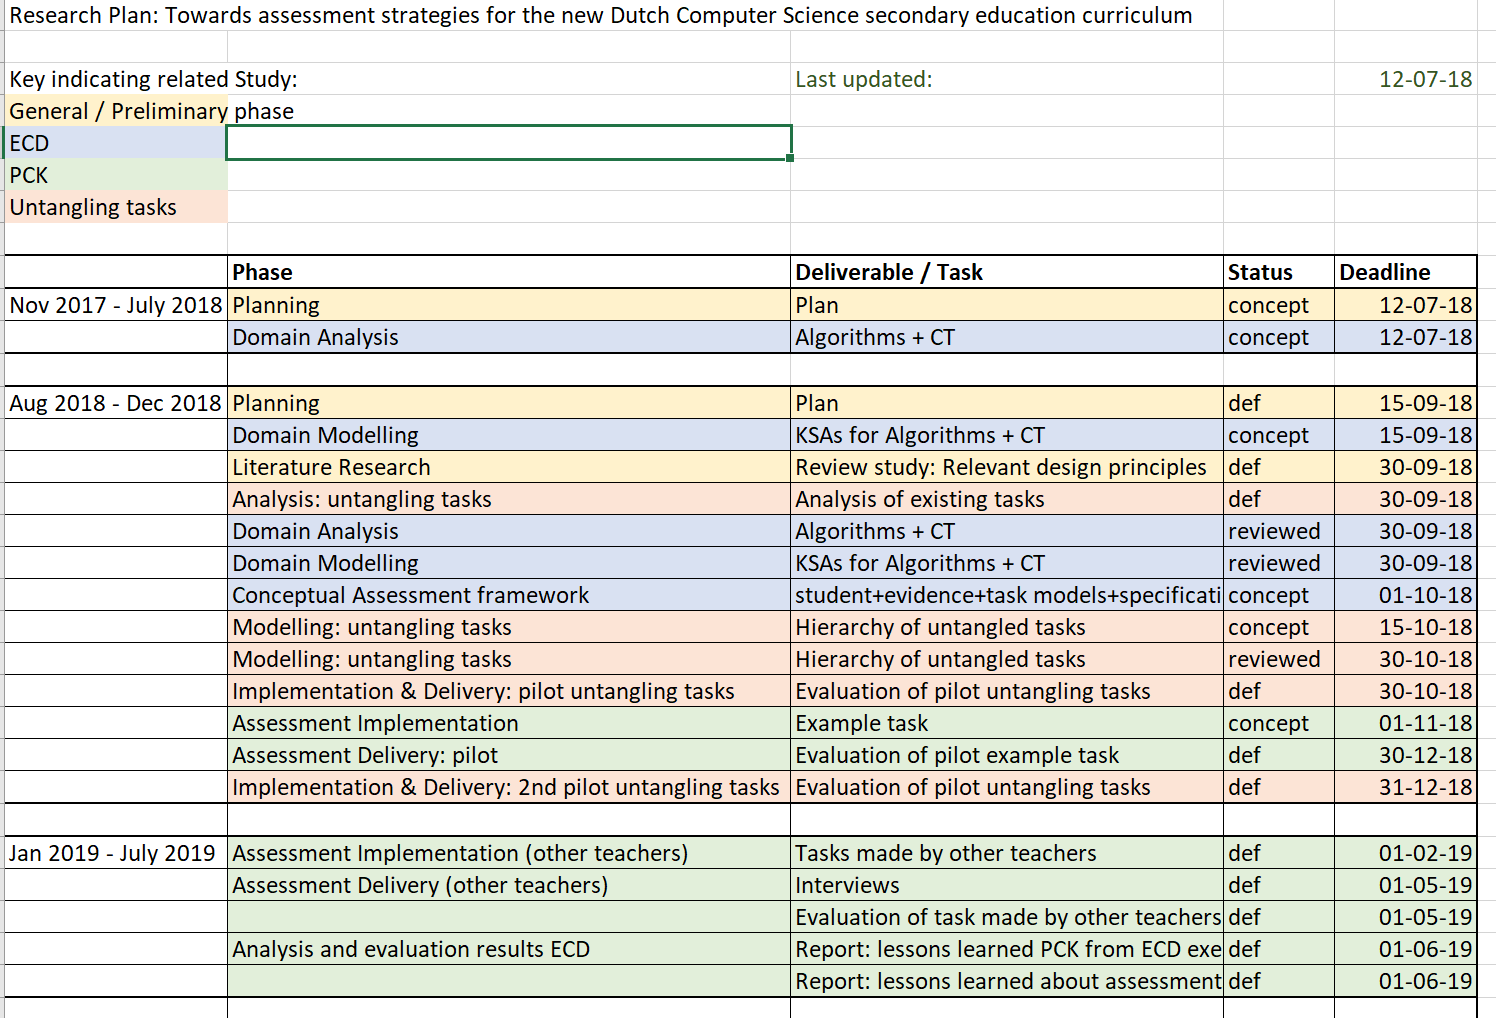
\includegraphics[scale=1.0]{figures/schedule.png}
%\caption{Schedule}\label{fig:schedule}
\end{sidewaysfigure*}


\section{Supervision}\label{sec:Supervision}

Prof. dr. Erik Barendsen (Radboud University, Faculty of Science) and dr. Jos Tolboom (SLO) will function as promoters.
As chair of the curriculum committee and advising on the implementation of the new curriculum Erik will \dots

As computer science curriculum developer, Jos will \ldots

The network of teachers designated to establishing new curriculum content is willing to cooperate.

%\section{Results}\label{sec:results}



%For this research we focus specifically on the level of understanding (the reading and tracing), and leave creating for further research. This set of assessment tasks could be used to adequately determine the mastery of a student for a specific aspect (for either a fundamental concept or a plan composition problem) and discover any alternative conceptions. In addition, it facilitates the identification of variable features.


%The assessments created by the teachers along with samples of their graded work will be analyzed in Atlas. In addition to semi-structured interviews, and teachers' notes on their thoughts and experiences during implementation will be used to investigate characteristics of PCK:
%\begin{itemize}
%\item experience using the design template (i.e., how much time they spent, if they encountered any problems, if they felt it was useful, if they felt they had sufficient knowledge and skills, what they used, what they didn't use)
%\item how they approached the task (i.e., how they started, what they did to overcome any hurdles),
%\item the quality criteria aspects discussed in section \ref{sec:qualityCriteria} (i.e. how satisfied are they about their own assessment),
%\item any suggestions for improvements.
%\end{itemize}



%This study starts with a literary review to inventory what is known about challenges that teachers face regarding assessment (as a part of PCK) in general, and pertaining to algorithms and algorithmic thinking in particular.
%
%
%The study continues with a document analysis of related work pertaining to assessment of CS concepts and skills. Research on existing assessment instruments and relevant international curricula are reviewed. To select the curricula, we first listed those curricula which have been referred to in recent publications. The next selection criteria pertained to the relevancy of the learning objectives. Those must coincide with the reformed Dutch curriculum, with a particular focus on algorithms or problem solving, as well as explicitly embedding Computational Thinking as a core competency. In the third selection, relevant supportive documentation was considered, such as progression pathways (CAS, corresponding to the national curriculum in the U.K.) or specific description of the KSA outcomes and mappings to their corresponding curricula (ECS and AP CS Principles as specifications of the U.S. CSTA, and AQA as specifications of the England national curriculum). This narrowed down to the following short-list of curricula: U.S. CSTA, the Israel nationwide CS curriculum, National curriculum for computing England, and the NCEA Digital Technologies curriculum in New Zealand. From these curricula, sample assessment tasks and the way in which they elicited evidence in relation to their KSAs was analyzed together with any available research generally describing the curriculum or specifically describing the development of assessments. In addition, relevant (inquiry based) tasks from Process Oriented Guided Inquiry Learning in Computer Science (CS-POGIL), the International Baccalaureate (IB) program, and the Computer Science Field Guide \cite{CSFieldGuide} were reviewed.
%
%
%Similar to the ECS, we use the structured ECD approach to establish a design template for assessments which can be fine-tuned by teachers to adhere to their own specific classroom needs. This structured approach results in a clear link between potential observations (evidence of students' knowledge or skills), evaluation procedures, and measurement models (see section \ref{sec:ECD}).\todo{evt rubrics etc}
%
%
%The design pattern is piloted in two stages. The results from literary review will be triangulated with teacher interviews and observations during the implementation and delivery phases in which teachers use templates to implement and deliver their customized assessments. Via qualitative analysis (teacher interviews, student think-aloud sessions, student self-evaluation, assessment task analysis, scoring process analysis) we seek to determine which characteristics in the design-patterns are feasible as PCK-enablers, and which aspects require refinement or further investigation (see also table \ref{table:MappingCriteriaMethod}). In an iterative process, the results are analyzed and evaluated, and the assessment instrument adjusted and refined. This process is repeated twice, first in a small-scale pilot, and then the candidate template assessment tasks will be deployed at multiple institutions for testing on a larger scale. We subsequently report our findings.




%
\section{Discussion}\label{sec:discussion}

Flowcharts are used to structure and guide the problem solving process of
programming. We summarize our findings according to the problem solving steps
presented in Section~\ref{sec:educationalMaterial}:

\subsubsection*{1. Abstract the problem from its description.}
    Unplugged activities help to understand the problem. Flowcharts are used to identify the relevant aspects in the problem description and model these in an abstract
    framework. This process supports communication in an early stage,
    facilitating brainstorming and tinkering. We see that having a
    plan increases self-efficacy, and gives students the confidence necessary to get started
    on a complex problem. A sketched flowchart
     provides means for peer-reviews and teacher feedback on the proposed
    solution. In addition, the high-level description helps abstract from
    details and focus on dealing with the problem instead of implementation details.

    Using the combination of unplugged and flowcharts, students seem more able to
    deal with more complex problems, come up with more creative solutions
    and run into less troubles in the process. It seems helps structure, develop
    and communicate thoughts and problem solving strategies prior to implementation.

    When dealing with more complex problems, students generally prefer
    creating high-level flowcharts to code. Our results suggest that students with
    prior programming experience are generally skeptical of using
    flowcharts. However, when flowcharts are introduced at an early stage
    and students are nurtured to use them habitually, we observe that
    students tend to have relatively less cognitive-load issues when
    dealing with more complex problems, despite their shorter programming
    experience. In our results, more summarization errors were made when directly
    implementing code than when using flowcharts. Omitting the last specified
    step in a goal (such as returning or printing a specific value)
    indicates that the students fail to maintain a bird's-eye view and
    loose sight of their goals.

\subsubsection*{2. Generate sub-problems.}
    As high-level flowcharts summarize the problem at hand, they seem to naturally
    facilitate design decomposition. Drawing a flowchart helps identify and recognize subproblems and divide the solution into more manageable chunks. For each subcomponent, the solution strategy and selection of plans is made and evaluated prior to implementation. Patterns and (obsolete) repetitions are recognized at an early stage. We suggest that sketching an idea in a flowchart and removing the burden of dealing with specific language constructs (syntax) lowers the cognitive load. It helps the student focus on finding an adequate approach to a problem.
     

    Our results suggest that going through the trouble of defining sub-methods
    in flowcharts leads to exactly those cognitive load-problems that
    flowcharts should help alleviate. Students experience making detailed
    low-level flowcharts as cumbersome and boring. A flowchart should be used as a method of abstracting from
    the details, not to further refine decomposed units. Creating a flowchart must remain practical, worth the effort and goal-oriented: high-level.


\subsubsection*{3. Transform sub-problems into sub-solutions.}
    With the design already
    thought-out, the student can focus specifically on
    coding details. Each flowchart component maps to a corresponding
    sub-method and is tackled individually. Students accurately and easily translate flowchart design into code.
    According to our observations, any mistakes in the design are adopted
    into code. This process, in which the student deals with the problem for
    a second time, does not lead to a reconsideration of the solution. Once
    students get into a doing mode, the thinking seems to stagnate. This
    emphasizes the need to think clearly before starting.

    Using Greenfoot's visually compelling environment each sub-solution
    is evaluated individually. The immediate visual feedback reinforces testing. If
    necessary, design or implementation adjustments are made. Learning
    problem solving skills and Java language constructs is thus
    interleaved with its application in an iterative think-act process.


\subsubsection*{4. Re-compose the sub-solutions into a working program.}

    The flowchart can be used as a road-map, guiding students through the
    composition of the sub-solutions into a complete solution.
 The algorithm that controls the sequence of
    events is implemented as specified by the flowchart. As the testing of the sub-solutions has been done
    thoroughly, this step is confined to reconsidering the manner in which sub-methods are interleaved. The
    result is tested and evaluated to ensure that the solution adheres to the requirements, reducing summarization errors.
      complete solution. If necessary (flowchart) design and coding steps are iterated.


    The implementation phase has thus been simplified to a direct translation from
    flowchart to code. The designed aspects, such as modularization and
    selection and application of plans (including abutment, nesting and merging) are
    automatically incorporated, yielding more structured, understandable and reusable code.

    Describing the initial and final states facilitates reasoning about
    sub-solution abutment (in addition to debugging). Moreover, it allows facilitates
    (JavaDoc) description of assumptions, requirements and pre and post conditions.
    The use of high-level flowcharts helps maintain a bird's eye view of the
    problem at hand, enabling students with solution evaluation: has the problem been solved?


\subsubsection*{5. Evaluate and iterate.}

    After having tested each individual sub-solution, the program as a whole is
    validated for correctness and completeness. Contrary to our experience with pure textual
    results, students generally don't give up until the result is exactly as proposed. The Greenfoot environment compels students to take appropriate action to fix any errors.

    Explicit attention should be given to reflection and evaluation in order to
    ensure that students learn from their mistakes through an iterative
    think-act process. This will help them learn from both construct-based and plan-composition
    errors.


\subsection*{Plans}
    Plans
    were taught explicitly, implicitly or not at all (see Section \ref{sec:courseObjectives}).
    \begin{itemize}[leftmargin=1em]
    \item Students had no problems understanding plans that were
        \emph{explicitly taught} in class.


    \item Students had no problems selecting the appropriate plan which was
        \emph{implicitly taught} through scaffolded assignments. However,
        CB errors were introduced during implementation and
        students tend to make errors when fine-tuning plans.


    \item Students could not apply a plan \emph{without prior instruction}
        or (scaffolded) practice.

    \end{itemize}


     Our results confirm de Raadt's call for
    teachers to teach plan-strategies explicitely\cite{deRaadt2008}. Based on the results mentioned above, we believe that students will perform
    better if they are appropriately introduced to different types of plans
    and practice applying them in different situations (i.e. selecting
    appropriate boundary values).


%\item \textbf{Choosing a plan}: At the end of the course students are
%    generally capable of choosing an appropriate plan and creating 'Correct
%    Idea' solutions using code and flowcharts for relational level
%    problems.



\subsection*{The role of coding}
    Coding gives students immediate feedback
    on their algorithms (in the role of a guide-by-an-expert). Students should be encouraged to actually code and run their algorithms.
    Lagging on homework leads to deficient fundamental construct-based
    knowledge, crucial to programming, such as assigning values to
    variables and understanding booleans. Working
    together with a picky compiler makes students aware of the need for
    precision. It helps
    them find, fix and learn from their own (logical) mistakes.


    Students rely on the computer to translate plans into correct and specific solutions. Whether syntax or logical errors, students solve these problems on their own during computer-assisted programming.

     \begin{description}[leftmargin=1em]

    \item[Syntax error detection:] Most of the CB errors made in
        the pen-and-paper assessments are syntax-related (such as
       '\jav{$=>$}'). The compiler helps detect and remove
        these. However, the pen-and-paper errors don't disappear over time.
        Students seem to be strongly reliant on compiler-assistance, and
        apparently, students don't internalize what the compiler is
        complaining about.


     \item[Evaluation:] Immediate (visual) feedback from the
         programming environment allows the students to test for plan
         composition problems, and adjust these where necessary. The result is a high success-rate.
         Our in-class observations indicate that students are highly motivated
         to keep going until the result is exactly as expected (or of even
         higher quality).



    In contrast to the paper-assessments, students never omit the testing
    phase during computer-assisted assignments. Whilst testing, students
    can recognize whether adequate boundaries have been chosen, and adjust
    these appropriately (possibly by trial-and-error). Even though
    paper-tests indicate an improvement over time, students continue to
    make logical errors. It seems as though the correction they make
     is not internalized. A more explicit reflection and evaluation phase
    may improve learning from mistakes. This is important, as logical errors are harder to detect in a less visual environment.



    \end{description}

\subsection*{Block-based systems}

Block-based systems, such as Scratch, Blockly, Alice, Greenfoot or
AppInventor are particularly successful among young novices. They help
abstract from concrete syntax, just like flowcharts. An advantage over
flowcharts is that they do not require an explicit coding step to convert to
an executable program. A disadvantage is that the instructions used are
low-level (just like Java statements themselves). For complex problems this
reduces to the same types of problems as code: students have no overview of
the complete program and poor design (such as lack of modularization).
Moreover, mastering text-based programming languages like Java or Python is
an enduring educational goal for students who wish to gain more in-depth
experience in coding.

Bridging the gap between the two editing styles (block-based and test-based)
appears to be difficult. In \cite{Kolling:2015} an intermediate style is
proposed: \emph{frame-based editing}. Frame-based editing, combines aspects
of blocks and text: on one hand it maintains the advantage of being less
syntax dependent, and on the other hand, it allows keyboard input.

The main problem with both frame-based and block-based systems is that
students are expected to use the computer right from the start. We observed
not only throughout the course of this study, but also in many other
programming courses, that the computer seems to cause students to switch from
a think-first-mode to an act-first-mode. The essence of our approach is to
keep students away from the computer so that they can focus on
problem-solving and design-aspects such as decomposition, instead of diving
into details (steps 1 and 2).


\subsection*{Improvements for the educational material}\label{sec:improvements}

\begin{description}[leftmargin=1em]

\item[Reflection:] Focus on \emph{iterating} between think-act and
    specifically incorporate \emph{evaluation}. To optimize the learning
    potential, teach students to reflect on what went wrong. This will help
    students understand logical boundary errors, syntax errors (such as
    those related to types and assignments) and increases their ability to
    re-use existing code. It should be emphasized that ad-hoc solutions may
    introduce new errors. If necessary, the flowchart should be adjusted
    accordingly.

\item[Flowcharts:] Establish concrete expectations about flowcharts, indicating:
    \begin{itemize}
    \item which details should be left out in a high-level flowchart;

    \item the role of initial and final state descriptions and how to use
        these in algorithmic thinking (sequencing of sub-methods);

    \item design rules in order to avoid arrow-spaghetti.
    \end{itemize}


\item[Tracing tables:] Introduce a structured approach for tracing
    variables in cognitively demanding situations such as loops and
    sub-methods.


\end{description}

%

\section{Conclusion and future work}\label{sec:conclusion}

The concepts of problem solving, algorithmic thinking and development of
programming solutions are closely related. Algorithm
design and a structured manner for problem solving become indispensable when
dealing with complex problems and their solutions.

The results of our primary exploratory case study seem to support our hypothesis. 
Thinking-first and planning ahead are important first steps in problem
solving. It requires a particular focus, we believe best achieved away from
the (distracting) computer. Selection of the suitable plan seems to benefit
from explicit instruction and 'thinking' before 'acting'. Algorithmic
thinking skills and a bird's-eye view are needed to link plans together to
create an adequate solution.


An appropriate plan to solve a problem (despite of any construct-based errors
introduced during implementation) has far more potential of leading to a
correct solution, than an incorrect plan which is implemented bug-free. Most
construct-based errors are syntax errors which the compiler will complain
about. However, logical errors are far more difficult to detect and fix. Plan
implementation is a cognitively demanding process: design, implementation and
testing of subtasks takes place while simultaneously considering the
high-level goals.

Flowcharts, and a stepwise approach to problem solving, can aid novice
programmers to keep track of where they are and give guidance to what they
need to do next, similar to how a road-map helps navigate. High-level
flowcharts aid decomposition, subtask recognition and lightens the cognitive
load (minimizing the errors arising from cognitive overload) as each subtask
is dealt with independently.


The exploratory case study that we conducted was small-scale. The material has been improved according to the annotations in section
\ref{sec:improvements}. The Dutch version is being published as official secondary school material for the Dutch national curriculum, and includes formative and summative tests. The English version will be made available through the Greenfoot website. We plan to carry out a \emph{follow-up study} in the course of this year. Student and teacher feedback while using the improved version will be collected and analysed. Feedback and new suggestions for improvements are to be incorporated in the following iteration. In addition, the following \emph{extensions} will be made:

%We will
%continue to teach the course over the next few years, both in high-school and
%as a freshman course in university. In addition, several teachers both
%nationwide and internationally have indicated that they use the course
%material in their classes. It would be interesting to carry out a follow-up
%study in which more data can be collected and analysed, yielding new
%suggestions for ongoing improvement of CS education.


%\renewcommand*{\bibfont}{\small}
%\bibliographystyle{ACM-Reference-Format}
%\bibliography{FlowchartsFirst}


\end{document} 